Consider an ellipse $\mathcal{E}$ and a fixed point $M$. Let $\mathcal{E}_n$ denote the {\em negative-pedal curve} with respect to $M$ \cite{stachel2019-conics}, i.e., the envelope of lines $\mathcal{L}(t)$ through a point $P(t)$ on $\mathcal{E}$ and perpendicular to $P(t)-M$; see Figure~\ref{fig:npc-3}. This article was motivated by a recent result  \cite{garcia2020-deltoid}: $\mathcal{E}_n$ is a three-cusp area-invariant deltoid for all $M$ on $\mathcal{E}$; see Figure~\ref{fig:npc-3} (top right).

\begin{figure}
    \centering
    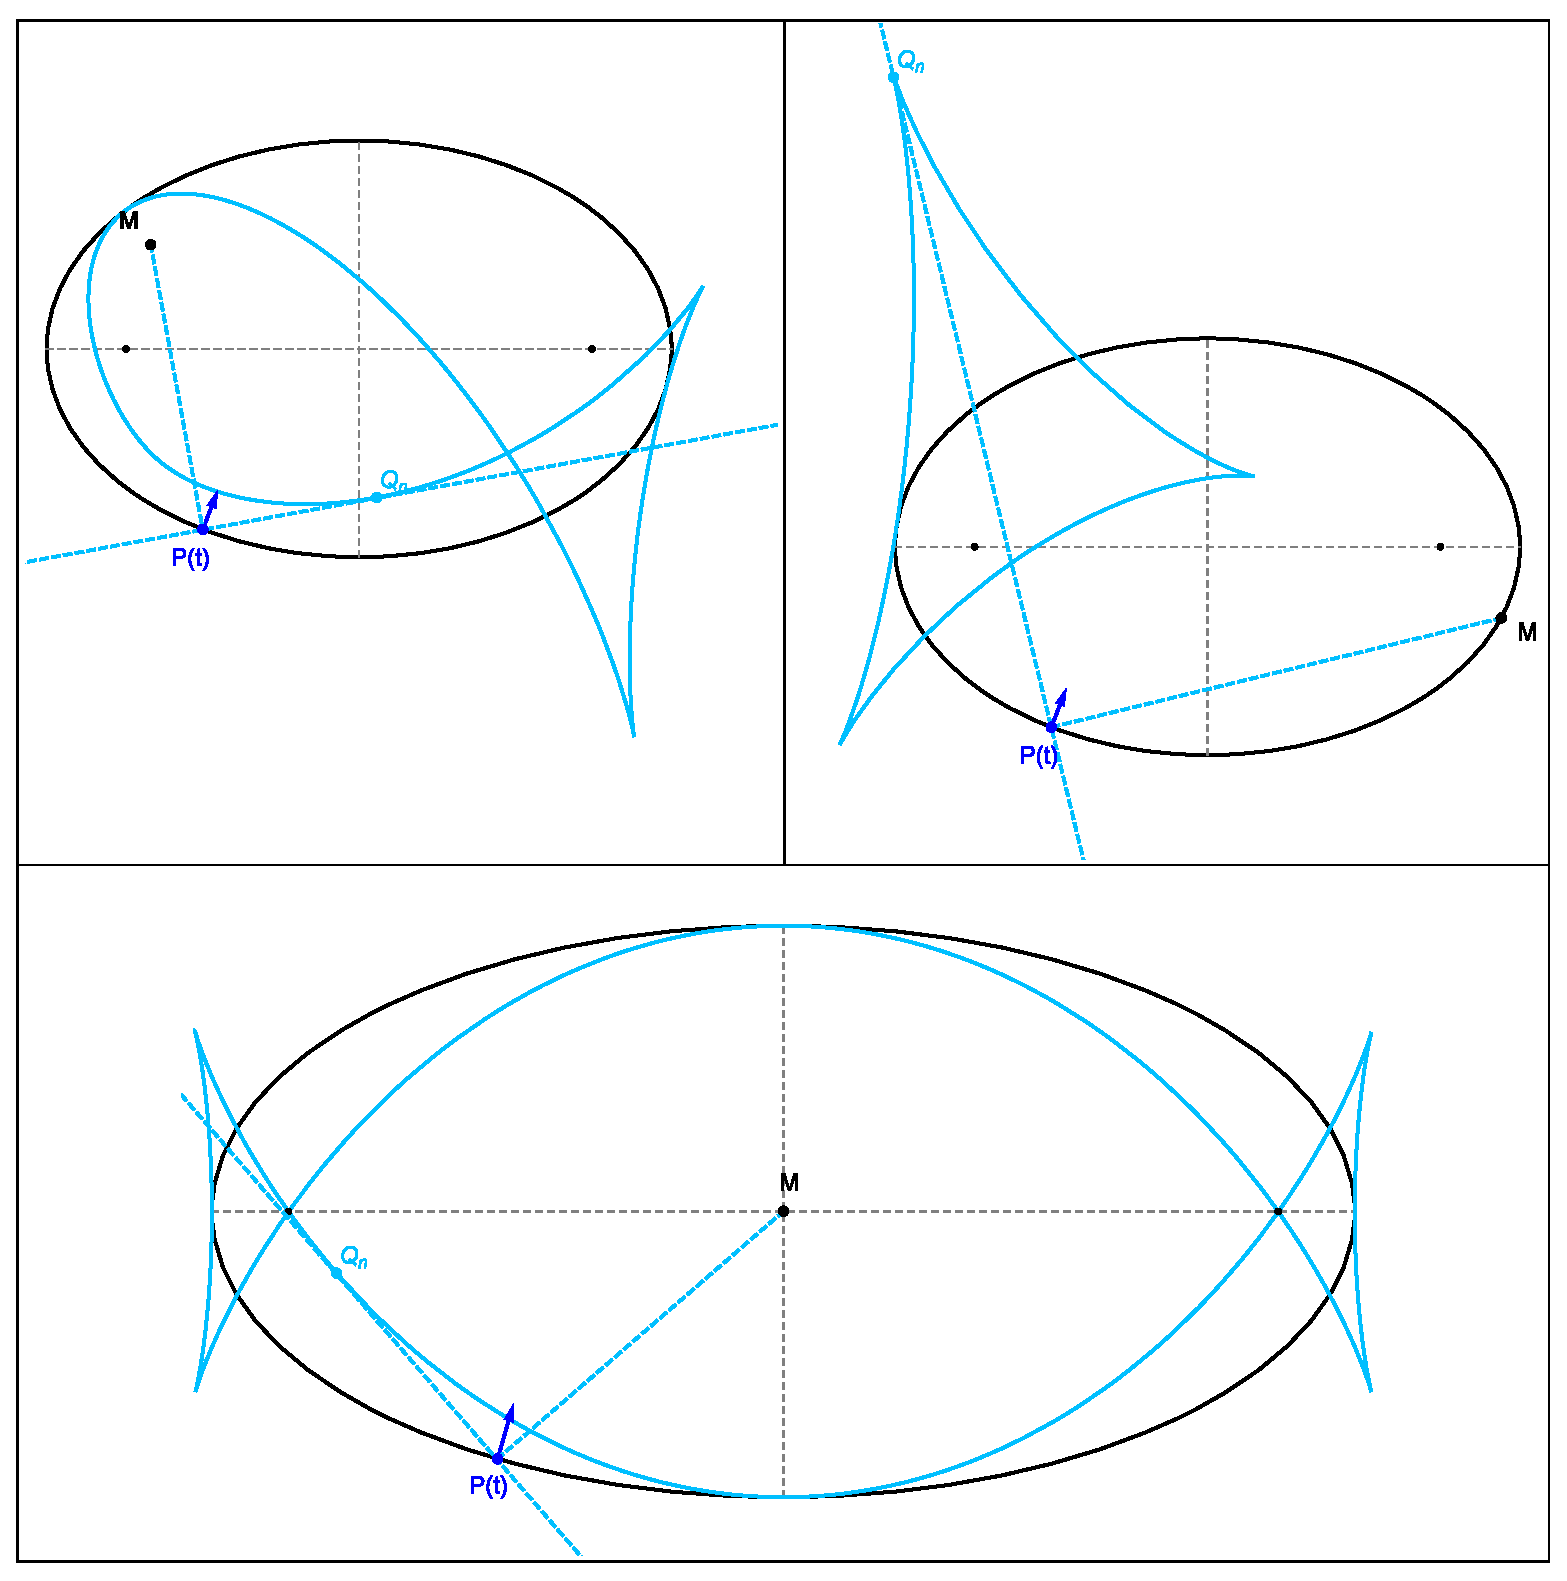
\includegraphics[width=\textwidth]{pics/0005_npc_3.eps}
    \caption{Examples of the Negative-Pedal Curve (light blue) of an ellipse (black) with respect to a point $M$. These are the envelope of lines through $P(t)$ on the ellipse, perpendicular to $P(t)-M$ ($Q_n$ is the tangent point). Three cases are shown, for $M$ (i) interior (top left), (ii) on the boundary (top right), and (iii) at the center (bottom) of the ellipse. For case (ii) the area of the curve is invariant for all $M$ \cite{garcia2020-deltoid}. Case (iii) yields Talbot's Curve \cite{mw} (in general it does not pass through the foci, but for the case shown, $a/b=2$, it does).} 
    \label{fig:npc-3}
\end{figure}

Let $\mathcal{E}_p$, $\mathcal{E}_c$ denote the {\em pedal}, and {\em contrapedal}, curves of $\mathcal{E}$ with respect to a point $M$ \cite{stachel2019-conics}; see Figures~\ref{fig:pedal-cp}. Recall the contrapedal of a plane curve is the pedal of the evolute \cite[Contrapedal]{mw}. For the ellipse, the evolute is a 4-cusp astroid \cite[Ellipse Evolute]{mw}; see Figure~\ref{fig:contrapedal}.  Additionally, define:

\begin{itemize}
    \item The {\em Rotated Pedal Curve} $\mathcal{E}_{\theta}$, the locus of foot $Q_{\theta}$ of a perpendicular dropped from $M$ onto the line through $P(t)$ oriented along a $\theta$-rotated tangent to the ellipse, Figure~\ref{fig:theta-mu}(left).
    \item The {\em Interpolated Pedal Curve} $\mathcal{E}_{\mu}$, the locus a point $Q_{\mu}=(1-\mu)Q_p+{\mu}Q_c$ ($\mu$ is a constant), i.e., an affine combination of pedal and contrapedal feet, Figure~\ref{fig:theta-mu}(right).
    \item The {\em Hybrid Pedal Curve} $\mathcal{E}^*$, the locus of the intersection $Q^*$ of $\mathcal{L}(t)$ with the line from $M$ to $Q_p$, Figure~\ref{fig:hybrid}.
    \item The {\em Pseudo Talbot Curve}\footnote{After the actual Talbot's Curve, shown in Figure~\ref{fig:npc-3} (bottom): the negative pedal curve of an ellipse with respect to its center $O$.} $\mathcal{E}^\dagger$, i.e., the Negative Pedal Curve of $\mathcal{E}^*$, Figure~\ref{fig:hybrid-npc}.
\end{itemize}

\begin{figure}
    \centering
    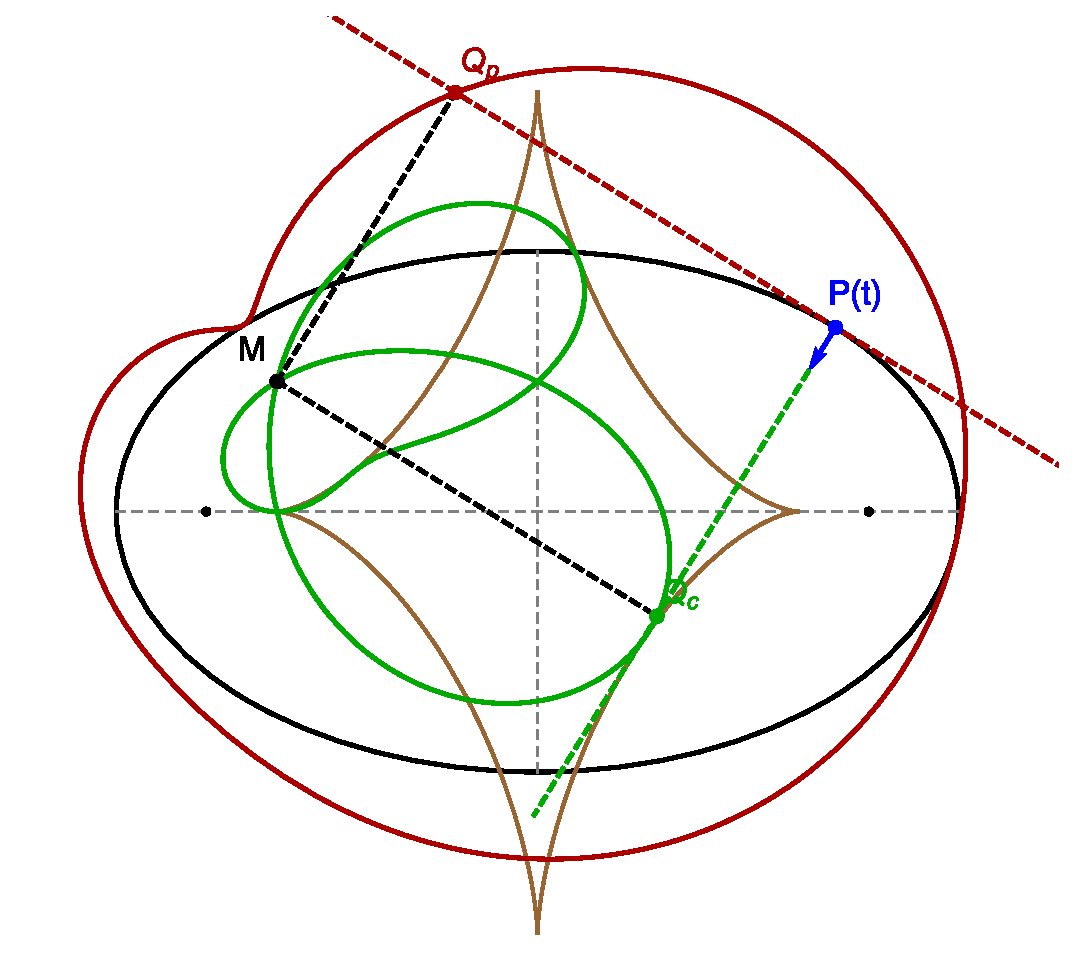
\includegraphics[width=.7\textwidth]{pics/0010_ped_cp.eps}
    \caption{The Ellipse Pedal Curve $\mathcal{E}_p$ (red) is the locus of the foot $Q_p$ of the perpendicular dropped from $M$ onto the line through $P(t)$ tangent to the ellipse. The Contrapedal Curve $\mathcal{E}_c$ (green) is the locus of foot $Q_c$ of the perpendicular dropped from $M$ onto the line through $P(t)$ normal to the ellipse. It can also be regarded as the pedal curve to the ellipse evolute (brown astroid).}
    \label{fig:pedal-cp}
\end{figure}

\begin{figure}
    \centering
    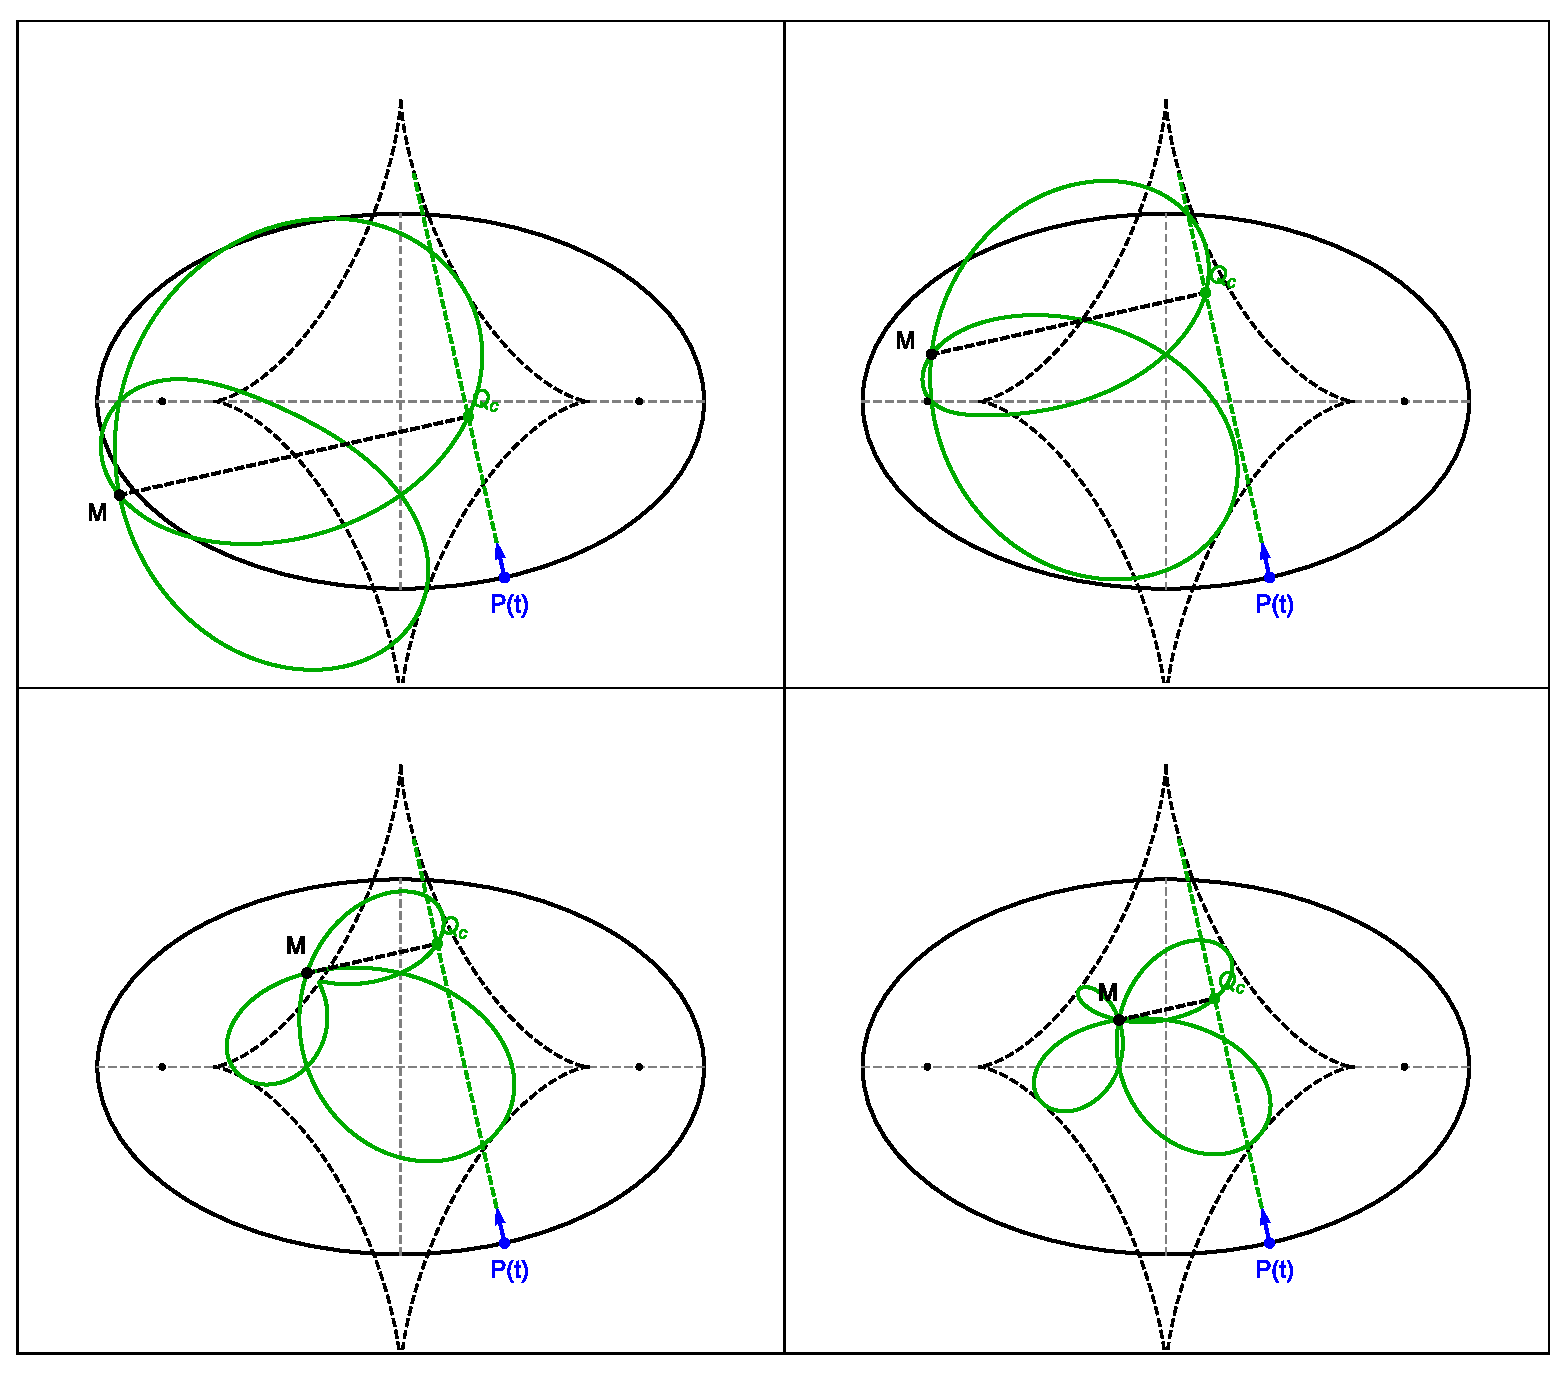
\includegraphics[width=\textwidth]{pics/0050_contrapedal_touchpts.eps}
    \caption{The ellipse Contrapedal Curve $\mathcal{E}_c$ (green) for four distinct positions of $M=[x_m,y_m]$. Notice the contrapedal is the pedal of the evolute (dashed black). We invite the reader to prove that (i) the curve's two self intersections (ignoring the one at $M$) always occur at $[x_m,0]$ and $[0,y_m]$ and (ii) that it touches the evolute at either 2 (top row) or 4 (bottom row) locations.}
    \label{fig:contrapedal}
\end{figure}

\begin{figure}
    \centering
    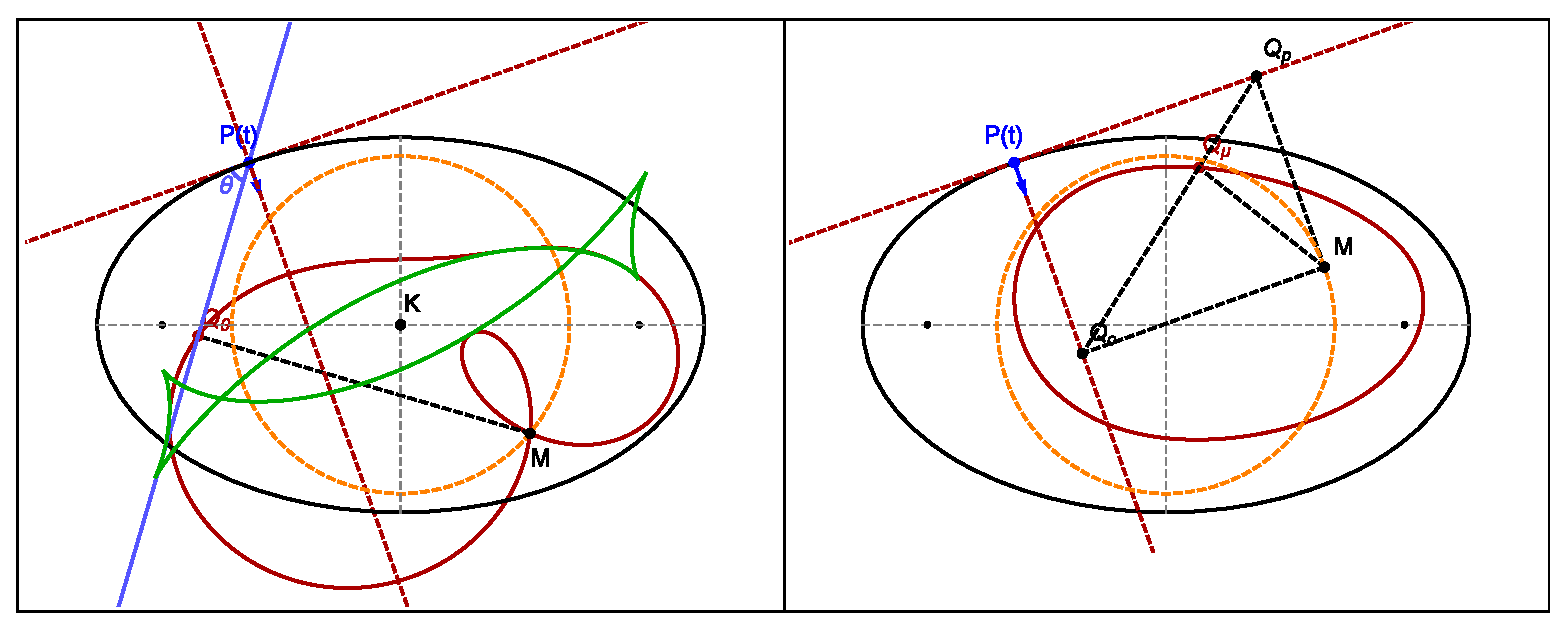
\includegraphics[width=\textwidth]{pics/0030_rot_mid.eps}
    \caption{\textbf{Left:} The rotated pedal curve $\mathcal{E}_{\theta}$ (red) is the locus of $Q_{\theta}$, the foot of a perpendicular dropped from $M$ onto a line through $P(t)$, along the $\theta$-rotated tangent (light blue), in this case $\theta=54^\circ$. $A_{\theta}$ is invariant for $M$ on a concentric circle (orange). Note $\mathcal{E}_0=\mathcal{E}_p$ and  $\mathcal{E}_{\pi/2}=\mathcal{E}_c$, and in general, $\mathcal{E}_\theta$ is the pedal curve with respect to the $\theta$-evolutoid (green), whose curvature centroid $K$ is stationary at $O$. \textbf{Right:} The interpolated pedal curve $\mathcal{E}_{\mu}$ (red) is the locus of $Q_{\mu}$, the affine combination of pedal $Q_p$ and contrapedal $Q_c$ feet, here $\mu=1/3$. $A_{\mu}$ is invariant provided $M$ lies on a concentric circle (orange).}
    \label{fig:theta-mu}
\end{figure}

Let $A$, $A_p$, $A_c$, $A_\theta$, $A_\mu$, $A^*$, and $A^\dagger$ denote the areas of $\mathcal{E}$, $\mathcal{E}_p$,
$\mathcal{E}_c$,
$\mathcal{E}_\theta$,
$\mathcal{E}_\mu$,  $\mathcal{E}^*$, and $\mathcal{E}^\dagger$, respectively. 

\subsection*{Main Results}

In Section~\ref{sec:review-steiner} we review a theorem by Jakob Steiner \cite{pamfilos2019-krummungs,steiner1838} concerning the Curvature Centroid (Krümmungs-Schwerpunkt) of polygons; a corollary is that $A_p$, $A_c$, and $A_{\theta}$ are invariant for $M$ along any circle concentric with $\mathcal{E}$. Furthermore, we prove $A_{\mu}$ also shares this property.

In Section~\ref{sec:explicit}, we derive explicit expressions for $A$, $A_p$, $A_c$, $A_\theta$, $A_\mu$ in terms of $\mathcal{E}$'s semi-axes $(a,b)$, $M$, $\mu$ and $\theta$. We also show that (i) $A_p-A_c=A$, and (ii) $A_p-A_\theta=A\sin^2\theta$.

In Section~\ref{sec:main-results} we prove that both $A^*$ and $A^\dagger$ are invariant for $M$ on $\mathcal{E}$. Finally, in Section~\ref{sec:epilogue}, we generalize area-invariance results to a large class of smooth curves. 

Appendix~\ref{app:general-evolutoids} contains  propositions supporting results related to ellipse evolutes and evolutoids (see \cite{jesus2015,jesus2014} for more details).
A table of all symbols used herein appears in Appendix~\ref{app:symbols}.

%\item Wherever $\mathcal{E}_p$ is tangent to $\mathcal{E}$, so is $\mathcal{E}^*$.
%\item $\mathcal{E}_c$ touches the ellipse evolute on either 2 or 4 points. \textcolor{red}{explicit conditions on $M$?}
% \item \textcolor{red}{ronaldo} $\mathcal{E}_c$ has two self-intersections at $(M_x,0)$, and  $(0,M_y)$.
    %\item \textcolor{red}{ronaldo} Let $C_{2,p}$ and $C_{2,c}$ denote the area centroids of $\mathcal{E}_p$ and $\mathcal{E}_c$, respectively. If $M$ moves along a circle, these move along ellipses.
    %\item The locus of $M$ for which $\mathcal{E}_p$ has a cusp is \textcolor{red}{...}



